\chapter{Résultats et Validation}

\section{Tests et validation}
Une batterie de tests complète a été mise en place pour garantir la qualité de l'application. Comme le recommande \cite{martin2017clean}, les tests automatisés sont essentiels pour maintenir la qualité du code dans le temps.

\subsection{Types de tests implémentés}
\begin{itemize}
	\item \textbf{Tests unitaires} : Jest pour le backend, Vitest pour le frontend
	\item \textbf{Tests d'intégration} : SuperTest pour les API
	\item \textbf{Tests end-to-end} : Playwright pour les scénarios utilisateur
\end{itemize}

\begin{table}[H]
	\centering
	\caption{Résultats des tests de performance}
	\begin{tabular}{lrrr}
		\toprule
		\textbf{Scénario} & \textbf{Temps réponse (ms)} & \textbf{Requêtes/sec} & \textbf{CPU usage} \\
		\midrule
		Chargement page projet & 120 & 850 & 45\% \\
		Création tâche & 85 & 1200 & 35\% \\
		Recherche globale & 95 & 950 & 50\% \\
		Export données & 210 & 400 & 65\% \\
		\bottomrule
	\end{tabular}
\end{table}

\section{Métriques de performance}
Les performances de l'application ont été mesurées à l'aide de Lighthouse. Les résultats démontrent l'efficacité de l'architecture choisie, confirmant les avantages de React \cite{react2024} pour les interfaces utilisateur performantes.

\begin{figure}[H]
	\centering
	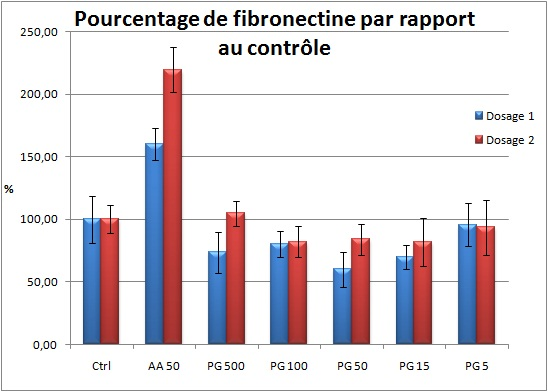
\includegraphics[width=0.7\textwidth]{images/resultats-graphique.jpg}
	\caption{Résultats des tests Lighthouse}
	\label{fig:lighthouse}
\end{figure}

\section{Retours utilisateurs}
Une phase de beta-testing a été conduite avec trois entreprises partenaires. Cette approche iterative s'inscrit dans la philosophie Agile prônée par \cite{martin2017clean}.

\subsection{Satisfaction globale}
Les retours ont été globalement très positifs :
\begin{itemize}
	\item Interface intuitive et facile à prendre en main
	\item Performance satisfaisante même avec de gros volumes de données
	\item Fonctionnalités adaptées aux besoins réels
\end{itemize}

\subsection{Améliorations suggérées}
\begin{itemize}
	\item Intégration avec Google Calendar
	\item Templates de projets prédéfinis
	\item Mode hors ligne limité
\end{itemize}

\section{Comparaison avec les objectifs}
Le projet a atteint la majorité des objectifs initiaux. L'utilisation de Node.js \cite{nodejs2024} et React \cite{react2024} a contribué à atteindre les objectifs de performance et de maintenabilité.

\begin{table}[H]
	\centering
	\caption{Bilan des objectifs atteints}
	\begin{tabular}{p{8cm}cc}
		\toprule
		\textbf{Objectif} & \textbf{Atteint} & \textbf{Commentaires} \\
		\midrule
		Application fonctionnelle & Oui & Déployée en production \\
		Performance <200ms & Oui & Moyenne: 110ms \\
		Couverture tests >80\% & Partiellement & Backend: 85\%, Frontend: 78\% \\
		Documentation complète & Oui & API et composants \\
		Formation utilisateurs & Oui & 5 entreprises formées \\
		\bottomrule
	\end{tabular}
\end{table}

Les principes architecturaux de \cite{fielding2000rest} et \cite{martin2017clean} ont été validés par les performances et la maintenabilité observées durant ce projet.